% 2017 全国Ⅰ卷 文6：选项 (A)(B) 的两个正方体
% 前面正方形 (0,0)-(2,2)，后面偏移 (0.85,0.5)；隐藏棱：后左竖棱、左底棱、后底棱
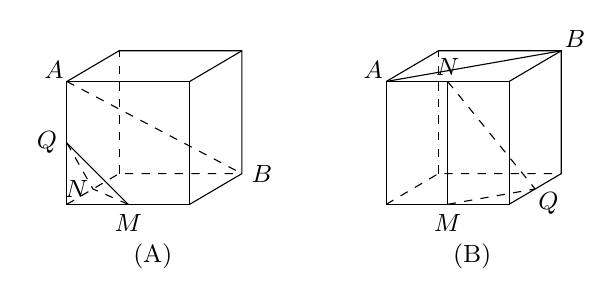
\begin{tikzpicture}[scale=0.78, font=\small]
  % ---------- (A)：A 前左上，B 后右下；M 前下棱中点，N 底面左棱中点，Q 前左竖棱中点 ----------
  \begin{scope}
    \draw (0,0) rectangle (2,2);
    \draw (2,0) -- (2.85,0.5) -- (2.85,2.5) -- (2,2);
    \draw (0,2) -- (0.85,2.5) -- (2.85,2.5);
    \draw[dashed] (0,0) -- (0.85,0.5) -- (2.85,0.5);
    \draw[dashed] (0.85,0.5) -- (0.85,2.5);
    \coordinate (A) at (0,2);
    \coordinate (B) at (2.85,0.5);
    \coordinate (M) at (1,0);
    \coordinate (N) at (0.425,0.25);
    \coordinate (Q) at (0,1);
    \draw[dashed] (A) -- (B);
    \draw (Q) -- (M);
    \draw[dashed] (Q) -- (N) -- (M);
    \node[above left, inner sep=1pt] at (A) {$A$};
    \node[right] at (B) {$B$};
    \node[below] at (M) {$M$};
    \node[left, inner sep=1.5pt] at (N) {$N$};
    \node[left] at (Q) {$Q$};
    \node at (1.4,-0.85) {(A)};
  \end{scope}
  % ---------- (B)：A 前左上，B 后右上；N 前上棱中点，M 前下棱中点，Q 底面右棱中点 ----------
  \begin{scope}[xshift=5.2cm]
    \draw (0,0) rectangle (2,2);
    \draw (2,0) -- (2.85,0.5) -- (2.85,2.5) -- (2,2);
    \draw (0,2) -- (0.85,2.5) -- (2.85,2.5);
    \draw[dashed] (0,0) -- (0.85,0.5) -- (2.85,0.5);
    \draw[dashed] (0.85,0.5) -- (0.85,2.5);
    \coordinate (A) at (0,2);
    \coordinate (B) at (2.85,2.5);
    \coordinate (N) at (1,2);
    \coordinate (M) at (1,0);
    \coordinate (Q) at (2.425,0.25);
    \draw (A) -- (B);
    \draw (N) -- (M);
    \draw[dashed] (N) -- (Q);
    \draw[dashed] (M) -- (Q);
    \node[above left, inner sep=1pt] at (A) {$A$};
    \node[above right, inner sep=1pt] at (B) {$B$};
    \node[above, inner sep=2pt] at (N) {$N$};
    \node[below] at (M) {$M$};
    \node[below right, inner sep=1pt] at (Q) {$Q$};
    \node at (1.4,-0.85) {(B)};
  \end{scope}
\end{tikzpicture}
